\documentclass[10pt,a4paper]{article}
\usepackage[margin=2cm]{geometry}
\usepackage[T1]{fontenc}
\usepackage{lmodern}
\usepackage{amsmath,amssymb}
\usepackage{booktabs}
\usepackage{graphicx}
\usepackage{caption}
\usepackage[hidelinks]{hyperref}
\graphicspath{{../results/}}
\captionsetup{font=small}
\setlength{\parskip}{3pt}

\title{Optimal Market-Neutral Pair Trading on Liquid Staking Tokens:\\
Ornstein--Uhlenbeck Spreads, EWMA Bands and DEX Frictions}
\author{AMOURETTE Pierre-Alexandre \quad DIJON Ilyes \quad FATHI Ayoub \quad REY Mathis\\[4pt]
\small Algorithmic Trading Project -- Extension of Yang \& Malik (2024)}
\date{November 2026}

\begin{document}
\maketitle
\vspace{-6mm}

\begin{abstract}
\noindent We adapt the Optimal Trading Technique (OTT) of Yang and Malik (2024) to three
liquid staking tokens (wstETH, rETH, weETH) priced in WETH on Uniswap~V3, with 1-hour
candles from the public GeckoTerminal API. We replace the empirical mean-reversion time
by an Ornstein--Uhlenbeck (OU) half-life, the fixed z-score by EWMA bands, and add fee
tiers, constant-product slippage and stochastic gas costs to the backtest and to the
optimisation. Out-of-sample, the strategy beats buy \& hold by 0.33~ETH on a 30~ETH book
without frictions, but with realistic frictions it does not trade at all at the observed
pool depth, and only earns 0.014~ETH when liquidity is assumed 50 times deeper.
\end{abstract}

%-----------------------------------------------------------------------
\section{Introduction and asset selection}

OTT is a multivariate pair-trading method. All pairs of a basket are tested for
cointegration, each spread generates open and close signals, and a bi-objective problem
(expected return minus $\lambda$ times risk) allocates capital among the pairs that signal
at the same time, under budget and market-neutrality constraints. The original study
trades ETH against fiat currencies on Kraken with a flat 0.1\% fee.

We apply the method to liquid staking tokens (LST). wstETH (Lido), rETH (Rocket Pool)
and weETH (ether.fi) are claims on staked ETH whose redemption value grows with the
staking yield. Each LST/ETH price therefore has a common economic anchor, close to
parity up to a slowly increasing exchange rate. The price differences between them come
from liquidity premia, redemption queues and order flow on thin pools. This makes
cointegration between LST prices plausible, while temporary deviations remain possible.
We trade only against WETH on Uniswap~V3 pools with an explicit fee tier. cbETH was in
the initial universe but was dropped: its most liquid pool had no swap in 72\% of the
hours, so its price was mostly stale.

%-----------------------------------------------------------------------
\section{Data and methodology}

\textbf{Data.} Hourly OHLCV candles and pool information (fee tier, TVL) come from the
public GeckoTerminal API. Pool addresses were found through its search endpoint. The free
API only serves the last 180 days of candles, so the requested window (Q4~2025--Q3~2026)
was not available. We use the most recent window: 1~June~2026 06:00 to
26~November~2026 23:00 UTC (179 days, 4\,290 hourly candles, cached in CSV for
reproducibility). The three pools all have a 0.01\% fee tier and TVLs of 2\,823 (wstETH),
308 (rETH) and 2\,131 (weETH) ETH, observed on 27~November~2026.

\textbf{Cleaning.} GeckoTerminal omits hours without a swap: 0.6\% of the hours for
wstETH, 20.4\% for rETH and 36.2\% for weETH. Prices are forward-filled for the spread
computation. However, a position is only opened or closed on a candle where both legs
had a real swap. A causal filter rejects any close more than 1\% away from the last
accepted close, unless the deviation persists for 3 consecutive candles (a genuine level
change). It removed 5 aberrant weETH prints. A minimum volume of 0.01~WETH per candle was
also tested and dropped, because it removed 8.5\% of the rETH and 14.0\% of the weETH
candles.

\textbf{Sample split.} The first 70\% of the candles (3\,003, up to 4~October~2026) are
in-sample (IS) and the last 30\% (1\,287) are out-of-sample (OOS). Regression, ADF and OU
parameters, and the entry threshold, are estimated on the IS only.

\textbf{Cointegration.} As in the paper, for each pair $(x,y)$ we regress the log-prices
by OLS and keep the residual spread
$s_t=\ln P^y_t-\beta\ln P^x_t-\alpha$ if an ADF test with constant and trend rejects a
unit root at 10\%. All three pairs pass (Table~\ref{tab:coint}).

\textbf{Portfolio and execution.} Each LST starts with an inventory worth 10~ETH (30~ETH
in total), mirroring the paper's capital per currency, so that the short leg sells tokens
already held (no borrowing). Opening a pair means selling the short LST for WETH and
buying the long LST with it (2 swaps); closing reverses the trade (2 swaps). The
portfolio is valued in ETH, and the benchmark is buy \& hold of the initial inventories.
The strategy is thus buy \& hold plus a market-neutral overlay. Signals use the close of
candle $t$ and data up to $t$. No new position is opened on a pair during its last $H$
candles (its OU half-life), because the spread would have no time to revert. Remaining
positions are closed on the last candle.

\begin{table}[h]
\centering\small
\caption{In-sample cointegration and OU estimates (time unit: one hour).}
\label{tab:coint}
\begin{tabular}{lrrrrr}
\toprule
Pair ($y$:$x$) & $\beta$ & ADF $p$-value & $\theta$ & Half-life $H$ (h) & $\sigma_{\text{eq}}$ (bp)\\
\midrule
rETH:wstETH  & 0.437 & 0.0009 & 0.057 & 12.2 & 7.5\\
weETH:wstETH & 1.064 & $<$0.0001 & 0.501 & 1.4 & 7.8\\
weETH:rETH   & 1.556 & 0.0015 & 0.120 & 5.8 & 16.0\\
\bottomrule
\end{tabular}
\end{table}

%-----------------------------------------------------------------------
\section{Mathematical formulation of the extensions}

\textbf{Ornstein--Uhlenbeck spread.} Each spread follows
$ds_t=\theta(\mu-s_t)\,dt+\sigma\,dW_t$. With a step of one candle, the exact
discretisation is the AR(1) $s_{t+1}=a+b\,s_t+\varepsilon_t$, estimated by OLS on the IS:
\[
\theta=-\ln b,\qquad H=\frac{\ln 2}{\theta},\qquad
\sigma^2=\operatorname{Var}(\varepsilon)\,\frac{2\theta}{1-b^2}.
\]
The half-life $H$ (in candles) replaces the paper's empirical average time to revert to
the mean. It is the holding horizon used for the expected gain and the risk of a pair.

\textbf{EWMA bands.} Let $m_t$ and $\mathrm{sd}_t$ be the exponentially weighted mean and
standard deviation of the spread (half-life 48~h). We use the deviation
$d_t=s_t-m_{t-1}$ and $z_t=d_t/\mathrm{sd}_{t-1}$, so only past data define the bands. A
position is opened when $|z_t|>k$: we long the spread (buy $y$, sell $x$) if $z_t<-k$ and
short it if $z_t>k$. It is closed when $z_t$ changes sign. Testing $k\in\{2,2.5,3\}$ on
the IS gave the same 5 trades with frictions for every $k$ (Sharpe 0.97). The tie is
broken by the IS Sharpe without frictions (6.88, 5.93, 4.84), so $k=2$.

\textbf{Expected gain and risk.} For a pair $n$ that signals at $t$:
\[
E_n=|d_t|\left(1-e^{-\theta H}\right),\qquad
V_n=\sigma^2\,\frac{1-e^{-2\theta H}}{2\theta}.
\]
$E_n$ is the expected move of the spread towards its EWMA mean over $H$ candles (half of
the deviation, since $H$ is the half-life). $V_n$ is the OU variance over the same
horizon. Unlike the paper, $E_n$ does not use the assets' drift: a pair trade earns the
reversion of the spread, not the trend of its legs. We also note an inconsistency in
the original formulation: its objective counts the short leg as $+|w_s|\,r_{\text{short}}$
and, combined with a negative $w_s$, its Hadamard-signed covariance also treats it as a
long position. We use signed long--short P\&L and variance instead.

\textbf{Optimisation.} With $w_n=w^{\ell}_n=-w^{s}_n$ the fraction of the initial
capital $C=10$~ETH traded on each leg, we solve with \texttt{cvxpy}:
\begin{align*}
\max_{w}\quad & \sum_n w_nE_n-\lambda\sum_n w_n^2V_n-\sum_n\left(w_nF_n+C\,w_n^2S_n\right)\\
\text{s.t.}\quad & 0\le w^{\ell}_n\le1,\quad -1\le w^{s}_n\le0,\quad w^{\ell}_n=-w^{s}_n,\quad
tw_c+\sum_{n:\,c\text{ sold}}|w^{s}_n|-\sum_{n:\,c\text{ bought}}w^{\ell}_n\le1,
\end{align*}
where $tw_c$ is the net fraction of asset $c$ already sold by open positions and
$\lambda=1$. Without frictions the last sum is dropped. With frictions, a round trip is
4 swaps, so $F_n=2(f_{\text{long}}+f_{\text{short}})$ (fee tiers) and
$S_n=2(1/R_{\text{long}}+1/R_{\text{short}})$ (slippage, below).

\textbf{Slippage.} A constant-product pool $x\,y=k$ with virtual reserves
$R=m\cdot\text{TVL}/2$ on each side (valued in ETH) returns, for an input $v$ net of
the fee $f$,
\[
\text{out}=\frac{R\,v(1-f)}{R+v(1-f)},\qquad
\text{loss}\approx\frac{v^2}{R}.
\]
The slippage is therefore quadratic in the trade size, which gives the term $C\,w^2S_n$.
The baseline is $m=1$. This is conservative, because Uniswap~V3 concentrates liquidity
around the peg and is much deeper near the current price than a full-range pool with the
same TVL. We therefore also report $m=10$ and $m=50$.

\textbf{Gas.} The gas price follows an OU process on its logarithm, simulated hourly
with a fixed seed:
$x_{t+1}=x_t+\kappa(\ln\bar g-x_t)+\sigma_g\varepsilon_t$, $g_t=e^{x_t}$, with
$\bar g=1$~Gwei (recent mainnet level), $\kappa=0.10$ per hour (spike half-life about
7~h) and $\sigma_g=0.30$. Over the OOS, the simulated gas has a median of 0.92~Gwei and a
5--95\% range of 0.32--2.83~Gwei. A swap costs $g_t\times150{,}000\times10^{-9}$~ETH.
Because gas is a fixed cost, it is checked after the optimisation: a trade of size
$v=wC$ is opened only if
$v(E_n-F_n)-S_nv^2>G$, where $G$ is the gas of 4 swaps at the median price.

%-----------------------------------------------------------------------
\section{Out-of-sample results}

The OOS runs from 4~October to 26~November~2026. Table~\ref{tab:res} reports the
total portfolio (30~ETH at the start, valued in ETH). The Sharpe ratio is annualised
from hourly returns with a zero risk-free rate (returns are in ETH). The \emph{win rate}
is the share of trades with a positive P\&L net of costs. \emph{Gain/loss} is the average
gain of winning trades divided by the average loss of losing trades (n/a without a
losing trade).

\begin{table}[h]
\centering\small
\caption{Out-of-sample performance (source: \texttt{results/metrics.csv}). $R\times m$:
slippage reserves $m\cdot$TVL/2.}
\label{tab:res}
\begin{tabular}{lrrrrrrrr}
\toprule
 & Final value & Return & Sharpe & Win rate & Gain/loss & Max DD & Trades & Avg size\\
 & (ETH) & (\%) & & (\%) & & (\%) & & (ETH)\\
\midrule
Buy \& hold            & 30.1730 & 0.58 & 2.78 & --   & --   & $-0.16$ & 0  & --\\
(a) No frictions       & 30.5033 & 1.68 & 4.97 & 100.0 & n/a & $-0.22$ & 39 & 7.45\\
(b) Frictions, $R\times1$  & 30.1730 & 0.58 & 2.78 & --   & --   & $-0.16$ & 0  & --\\
(b) Frictions, $R\times10$ & 30.1730 & 0.58 & 2.78 & --   & --   & $-0.16$ & 0  & --\\
(b) Frictions, $R\times50$ & 30.1873 & 0.62 & 2.67 & 77.8 & 0.91 & $-0.15$ & 9  & 2.23\\
\bottomrule
\end{tabular}
\end{table}

\textbf{Without frictions}, the overlay adds 0.33~ETH to buy \& hold with 39 winning
trades out of 39 (14 on rETH:wstETH, 17 on weETH:wstETH, 8 on weETH:rETH). It raises the
Sharpe ratio from 2.78 to 4.97. Buy \& hold already has a high Sharpe ratio, because LST
prices in ETH accrue the staking yield with very low volatility. \textbf{With frictions at
the observed depth} ($m=1$ and $m=10$), no trade is opened. Either the expected gain is
below the fee rate, so the optimiser sets $w=0$ (61 and 47 signals), or, at the size
where slippage balances the gain, the net gain does not cover the round-trip gas (38 and
52 signals). Only with 50 times deeper reserves does the strategy trade: 9 trades of
2.23~ETH on average, 7 of them winning, for +0.014~ETH over buy \& hold. The Sharpe ratio
is slightly lower than buy \& hold (2.67), because the overlay adds variance.

The rule that both legs must have a real swap matters for these illiquid pools. Out of
sample, it skipped 15 entry signals and delayed 16 exits in variant (a), and it skipped
73 entry signals in variants (b) with $m=1$ and $m=10$ (34 entries skipped and 9 exits
delayed with $m=50$). The end-of-sample rule skipped 2 entries in every variant.

\begin{figure}[t]
\centering
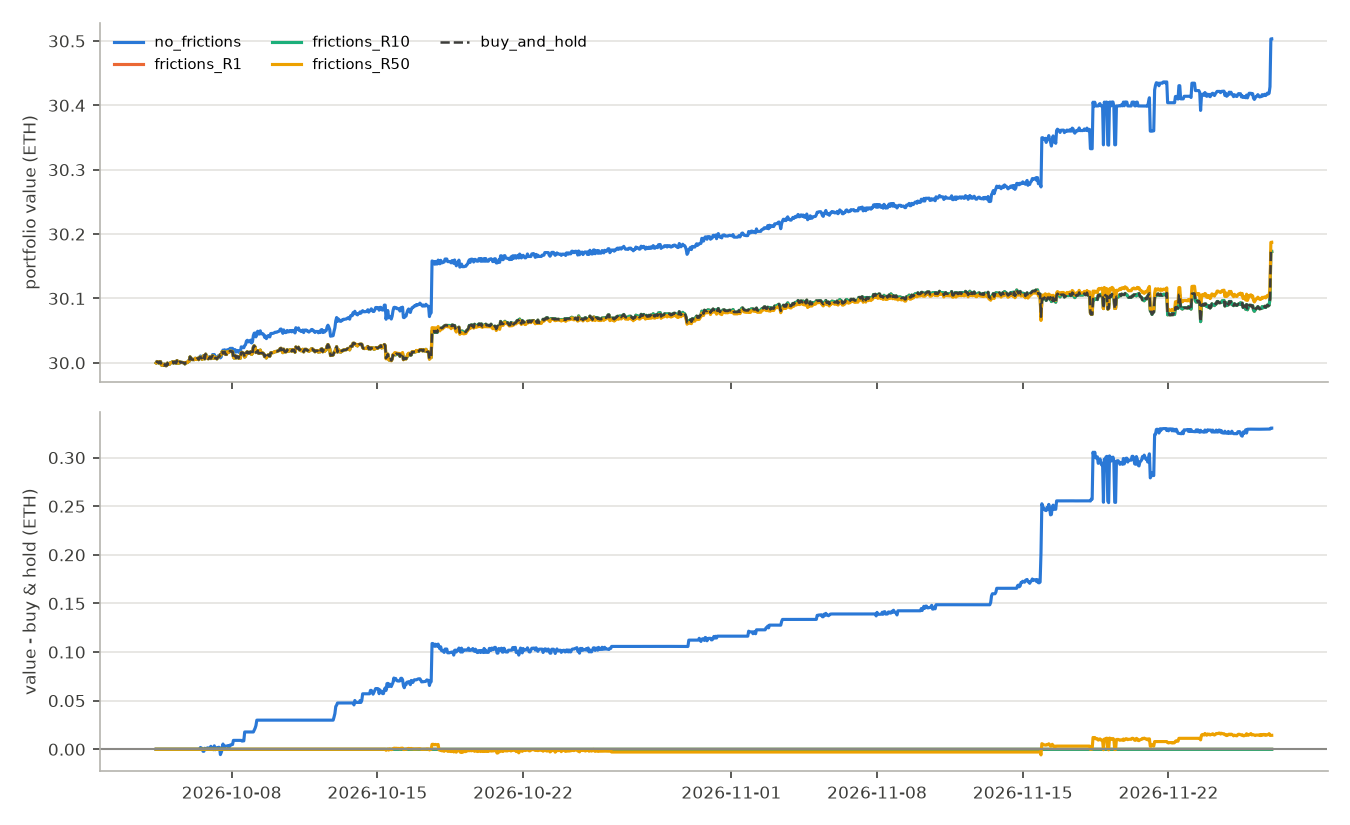
\includegraphics[width=0.8\textwidth]{equity_curves.png}
\caption{Portfolio value (top) and difference to buy \& hold (bottom), out-of-sample.
$R\times1$ and $R\times10$ do not trade and coincide with buy \& hold.}
\label{fig:equity}
\end{figure}

\begin{figure}[t]
\centering
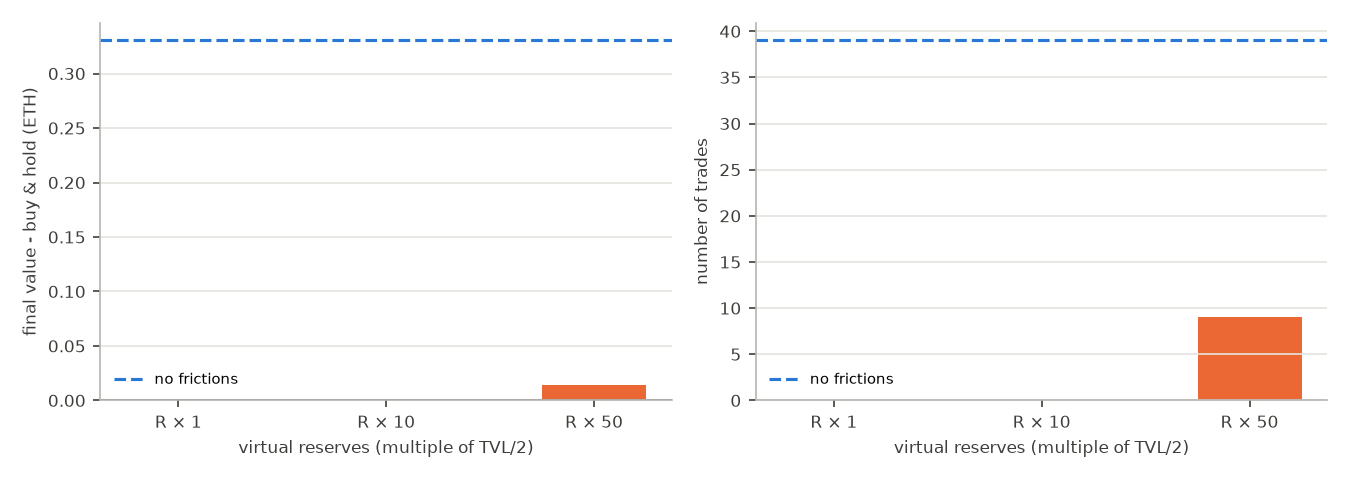
\includegraphics[width=0.7\textwidth]{slippage_sensitivity.png}
\caption{Slippage sensitivity: final value minus buy \& hold (left) and number of
trades (right) as a function of the virtual reserves; dashed line: no frictions.}
\label{fig:sens}
\end{figure}

\begin{figure}[t]
\centering
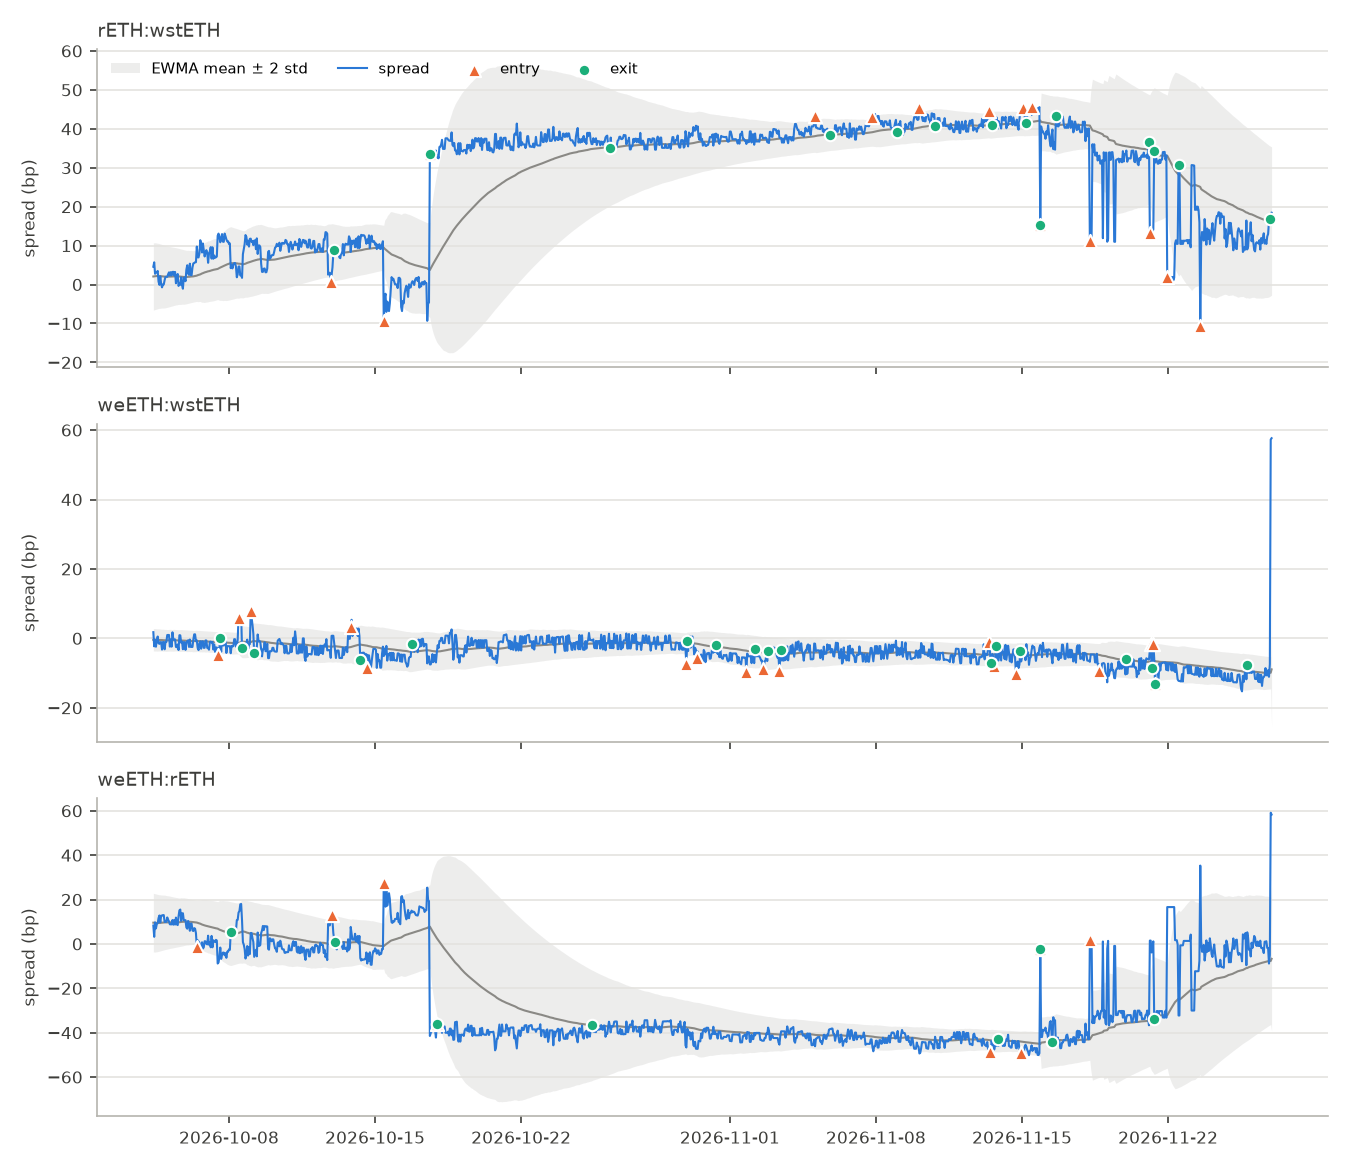
\includegraphics[width=\textwidth]{spreads_no_frictions.png}
\caption{Out-of-sample spreads (bp) with EWMA mean $\pm2$ std and the entries/exits of
variant (a).}
\label{fig:spreads}
\end{figure}

%-----------------------------------------------------------------------
\section{Limitations and conclusion}

\textbf{Infrequent and noisy prices.} rETH and weETH have no swap in 20\% and 36\% of the
hours. Forward-filled prices can create artificial mean reversion. The 1.4~h half-life of
weETH:wstETH probably reflects microstructure noise as much as true reversion. The rETH
spreads also jump to new levels (about $+30$~bp on 17~October) and flicker between two
levels after 15~November (Figure~\ref{fig:spreads}). The largest steps of the frictionless
equity curve coincide with these jumps, so part of the gain comes from thin-pool prints
that may not be tradable. Finally, a single 0.0002~WETH weETH swap on 26~November at
22:00 printed $+0.68\%$, below our 1\% filter. It raises every portfolio value, buy \&
hold included, by about 0.07~ETH on the last two candles (visible at the end of
Figure~\ref{fig:equity}), but leaves the comparisons almost unchanged.

\textbf{Risk aversion barely binds.} With $\lambda=1$, the risk term $\lambda V_n$ is
two to three orders of magnitude smaller than $E_n$, so sizing is driven by the
budget constraint (no frictions) or by slippage (with frictions). Calibrating $\lambda$
on the IS is left for future work. Moreover, because $H$ is the half-life,
$E_n=|d_t|/2$ and $V_n=\tfrac34\sigma_{\text{eq}}^2$ for every pair. The OU speed sets
the horizon, but the value of $\theta$ itself has little influence on sizing.

\textbf{Conservative slippage and other simplifications.} The $x\,y=k$ model on TVL/2
ignores concentrated liquidity, so the $m=1$ case overstates price impact. The TVL is a
single snapshot (27~November~2026) applied to the whole sample. Trades execute at the
signal candle's close, without latency, MEV or failed transactions. The OOS covers only
53 days and 1\,287 hours, and the window is constrained by the free API.

\textbf{Conclusion.} OU half-lives and EWMA bands produce a frictionless overlay that is
consistently profitable on LST spreads: 39 winning trades and +0.33~ETH over buy \& hold
on 30~ETH in under two months. But the spreads have a stationary standard deviation of
only 7--16~bp, so the expected reversion per trade is of the same order as the 4~bp of
round-trip fees plus gas. On pools as shallow as the rETH one, constant-product
slippage removes the opportunity entirely. A realistic evaluation therefore needs a
concentrated-liquidity price-impact model and deeper venues before the strategy can be
considered implementable.

\vspace{2mm}
\noindent{\small\textbf{Reference.} Yang, H., \& Malik, A. (2024). Optimal market-neutral
multivariate pair trading on the cryptocurrency platform. \emph{International Journal of
Financial Studies}, 12(3), 77.}

\end{document}
